\section{Partitioning the data}

\frame{\frametitle{Subsets in the data}
    Traditional methods include~\footfullcite{Nolte2003}:

    \begin{itemize}
        \item condition-specific populations
        \item segmenting by age
    \end{itemize}

    However, these methods have the common flaw of under-representing groups of
    healthcare users~\footfullcite{Vuik2016}.
}

\frame{\frametitle{Misrepresentation}
    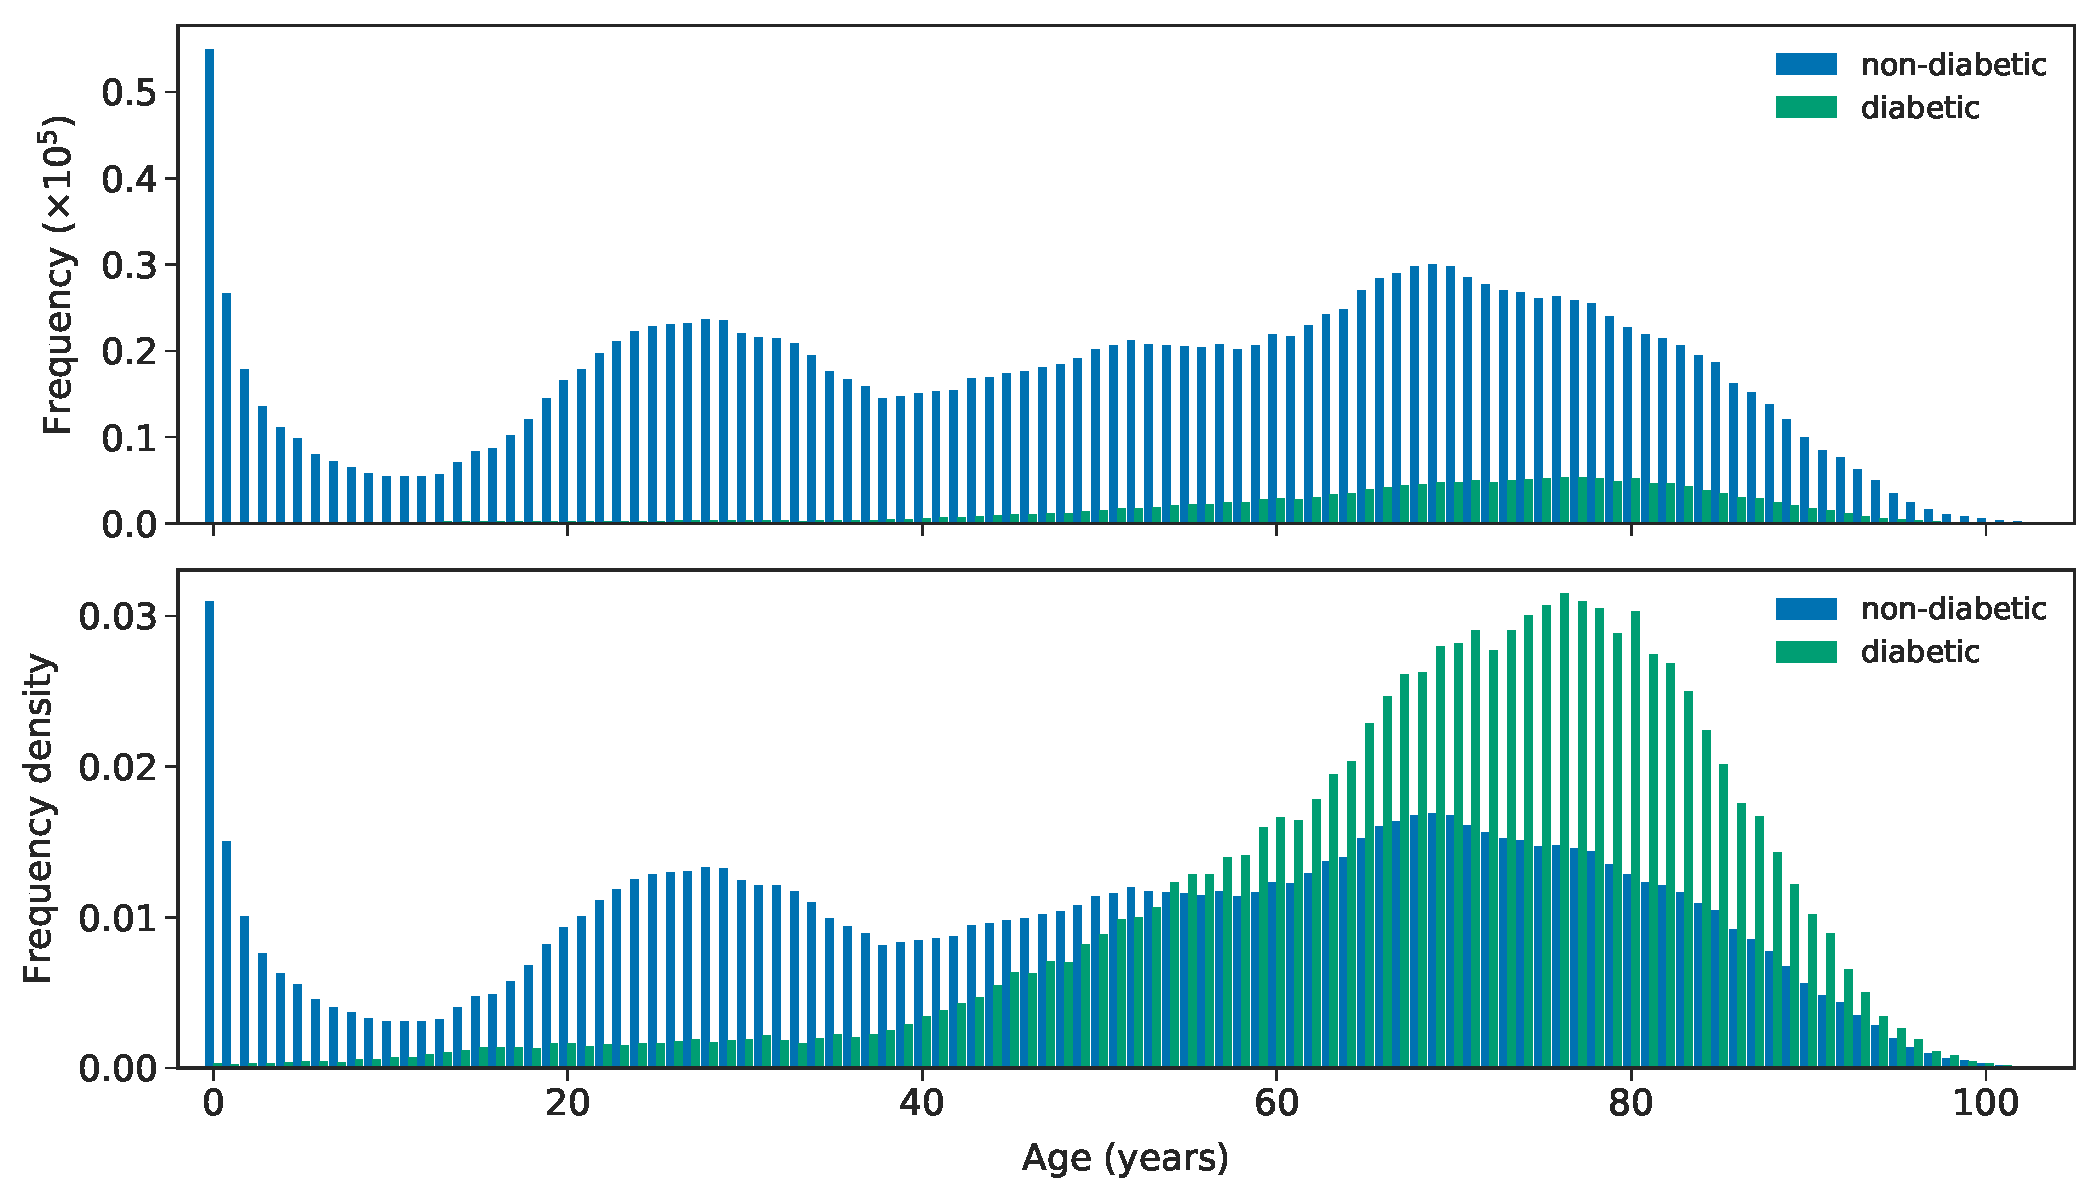
\includegraphics[width=\linewidth]{age_bar.pdf}
}

\frame{\frametitle{Misrepresentation}
    \resizebox{\textwidth}{!}{%
        \begin{tabular}{llllll}
\toprule
{} & Non-diabetic &    Diabetic & Diabetic under 30 & Diabetic 30 to 65 & Diabetic 65 and over \\
\midrule
mean &     1,647.00 &    2,648.98 &          1,335.11 &          2,110.79 &             2,940.21 \\
std  &     3,019.53 &    4,152.20 &          2,034.58 &          3,565.45 &             4,415.44 \\
min  &         4.50 &       10.91 &             52.48 &             35.93 &                10.91 \\
1\%   &        62.55 &      139.65 &            125.54 &            129.63 &               143.83 \\
25\%  &       338.67 &      490.64 &            431.76 &            404.30 &               546.11 \\
50\%  &       709.32 &    1,227.95 &            840.28 &            990.53 &             1,395.78 \\
75\%  &     1,756.90 &    3,106.44 &          1,605.21 &          2,338.76 &             3,584.18 \\
95\%  &     6,179.79 &    9,591.06 &          3,698.95 &          7,551.34 &            10,457.59 \\
99\%  &    13,414.48 &   19,128.45 &          7,697.49 &         16,277.28 &            20,310.51 \\
max  &   369,168.93 &  273,450.30 &         66,963.80 &        106,860.69 &           273,450.30 \\
\bottomrule
\end{tabular}

    }
}

\graphicspath{{img/clustering/}}
\frame{\frametitle{What is clustering?}
    \begin{figure}[htbp]
        \centering
        \animategraphics[loop,
                         controls,
                         width=.5\imgwidth]{1}{kmeans-}{0}{12}
    \end{figure}

    \footnotesize Image taken from \url{%
        https://www.jeremyjordan.me/
        grouping-data-points-with-k-means-clustering/
    }
}

\frame{\frametitle{Clustering with healthcare data}

    \small{%
    \begin{itemize}
        \item \fullcite{Kalyani2012}
        \item \fullcite{Rebuge2012}
        \item \fullcite{Vuik2016}
    \end{itemize}
    }
}

